\documentclass[12pt]{article}
\usepackage[margin=1in]{geometry}
\usepackage{amsmath, amsfonts, amssymb}
\usepackage{graphicx}
\graphicspath{{./images/}}
\usepackage{hyperref}
\usepackage{color}
\usepackage{multirow}
\usepackage{booktabs}   
\usepackage{adjustbox}
\usepackage[
backend=biber,
style=alphabetic,
]{biblatex}
\addbibresource{references.bib}

% Define red alert TODO
\newcommand{\todo}[1]{\textcolor{red}{TODO: #1}}

\title{V1}
\author{Chunyu Yang}
\date{\today}

\begin{document}
\maketitle

\section{Introduction}

The rapid proliferation of non-geostationary orbit (NGSO) satellite constellations, driven by advancements in low-cost launch technologies and the demand for global broadband connectivity, has intensified the risk of co-frequency interference with geostationary orbit (GSO) systems. For instance, large-scale NGSO constellations like Starlink and OneWeb share overlapping frequency bands with critical GSO services such as fixed-satellite (FSS) and broadcasting-satellite (BSS) systems, creating unprecedented challenges in spectrum coexistence. The International Telecommunication Union (ITU) underscores the urgency of interference mitigation in Radio Regulation, which mandates that NGSO systems "shall not cause unacceptable interference to geostationary-satellite networks" while imposing stringent limits on equivalent power flux density (EPFD) and off-axis emissions. These regulations aim to protect GSO operations, such as weather monitoring and telecommunications, which underpin vital global infrastructure.



\section{System Model}

This study explores the downlink dynamics of forward links originating from two distinct satellite constellations. We focus primarily on satellites in geostationary orbit (GSO), serving as the main communication system. Satellites in non-geostationary orbit (NGSO), particularly those in low Earth orbit (LEO), are considered potential sources of interference to a general GSO ground station (GGS). In this section, we provide a comprehensive description of the system model, which encompasses link budget calculations and the modeling of the received digital baseband signal, shown in \autoref{fig:interference-scenario}

\begin{figure}[htbp]
    \centering
    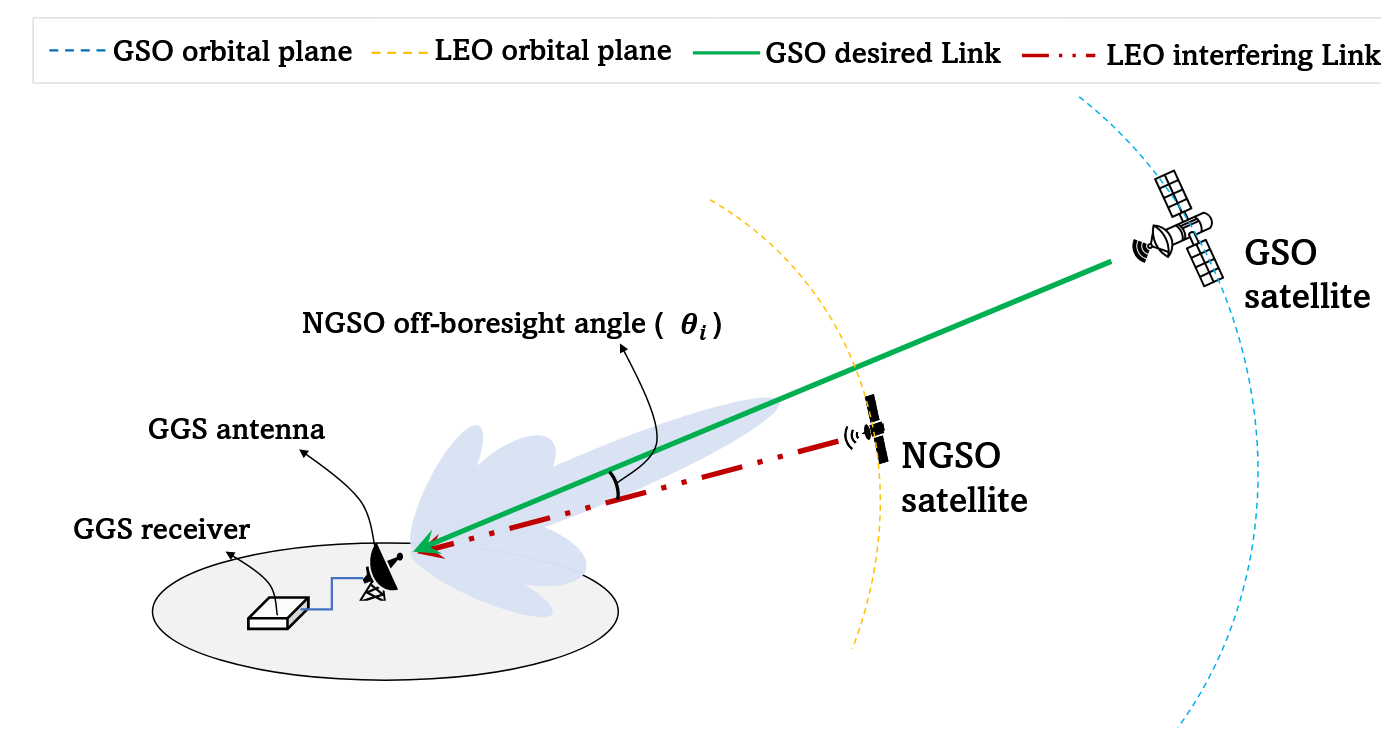
\includegraphics[width=0.9\textwidth]{ngso-gso-interference.png}
    \caption{Interference model where the primary system is GSO satellites and the interference source is LEO satellites.}
    \label{fig:interference-scenario}
\end{figure}

\subsection{Link Budget Model}

In our analysis, both GSO and LEO satellites are actively transmitting signals, with their main transmission lobes consistently directed toward a GGS. At the GGS receiver, the carrier power received from the desired GSO satellite system can be calculated using the following equation:
$$
    C = \frac{\text{EIRP}_{\text{gso}} \times G_{\text{r, gso}(\theta_0)}}{L_{\text{FS, gso}} \times  L_{\text{add}}}
$$
where $C $ is the received carrier power, $\text{EIRP}_{\text{gso}}$ is the equivalent isotropic radiated power of the GSO satellite, $G_{\text{r, gso}(\theta_0)}$ is the maximum receive antenna gain of the GGS, with $\theta_0$ being the boresight angle. $L_{\text{FS, gso}}$ is the free space path loss (FSPL) between the GSO satellite and the GGS. $L_{\text{add}}$ accounts for additional losses in the link, such as atmospheric and environmental losses.

As LEO satellites traverse the visible sky from the GGS, the station may concurrently receive signals from one or more LEO satellites, especially when they operate in the same frequency bands as the GSO satellite. These LEO signals can elevate the interference level within the primary signal. The interference power $I_k$ received from an individual LEO satellite indexed by $k$ is calculated as:
$$
    I_k = \frac{\text{EIRP}_{k} \times G_{\text{r, k}}(\theta_k) \times B_{\text{adj, k}}}{L_{\text{FS, k} }\times  L_{\text{add}}}
$$
where $B_{\text{adj, k}}$ is the adjustment factor accounting for bandwidth overlap between the GSO and LEO signals, with a value between 0 and 1.

The downlink carrier-to-noise ratio (CNR) of the GSO satellite signal received by the GGS is calculated as:
$$
    \text{CNR} = \frac{C }{k_{\text{boltz}}TB}
$$
where $k_{\text{boltz}}$ is the Boltzmann constant, $T$ is the receiver noise temperature., and $B$ is the bandwidth of the GSO baseband signal.

Similarly,  the interference-to-noise ratio (INR) received from the $k$th LEO satellite is:
$$
    \text{INR}_k = \frac{I_k }{k_{\text{boltz}}TB}
$$

To evaluate the effect of interference from all LEO satellites, we use the carrier-to-interference-plus-noise ratio (CINR):
$$
    \text{CINR } = \frac{C }{\sum_{k=1}^{K }I_k + k_{\text{boltz}}TB}
$$
where $K$ is the total number of interfering LEO satellites at a given time.

\subsection{Received Signal Model}

The total received signal at the GGS is the sum of the desired signal, interference from all LEO satellites, and additive white Gaussian noise (AWGN):

$$
    y(t ) = x(t ) \sqrt{\text{CNR }} + \sum_{k=1}^{K } \left(i_{k}(t )e^{j 2 \pi (f_{\text{c, k}}- f_{\text{c, gso}})t} \sqrt{\text{INR }_{k}}\right) + \zeta(t)
$$
where $x(t)$ is the baseband signal trasmitted by GSO satellite, $i_{k}(t)$ is the interfering signals from the $k$th LEO satellite.
At give time t, there are $K$ interfering LEO satellites, the carrier frequencies of the $k $th LEO satellite and the GSO satellite are $f_{\text{c, k}}$ and $f_{\text{c, gso}}$ respectively. The exponential term accounts for the frequency difference .

For further analysis and potential machine learning applications, the received signal can be represented in both time and frequency domains:
\begin{enumerate}
    \item Time-domain representation: The amplitude of $y(t)$ is sampled to create a one dimensional sequence $y^{A}$.
    \item Frequency-Domain Representation: The power spectral density (PSD) of $y(t)$ is estimated using Welch's method, which divides the signal into overlapping segments and computes the periodogram of each segment, resulting in one dimensional $y^{F } = 10 \log_{10}(\phi(y(t )))$
\end{enumerate}

\section{Proposed Deep Learning Models}

This section presents a novel framework for multi-modal interference detection in satellite communication, leveraging both time domain and frequency domain data. Three classes of deep learning models are proposed: Autoencoders(AE), Variational Autoencoders(VAE), and Conditional Variational Autoencoders(CVAE). Each class is implemented with three architectural variants: linear, convolutional and transformer based, to explore the impact of feature extraction mechanisms. The core innovation lies in fusing time and frequency information to anomaly detection robustness.

Next, we seek to define a reliable reconstruction error threshold. This threshold will then be applied to signals, regardless of interference. If the detected error values surpass this set threshold, interference is identified.

We denote the time and frequency domain signal input as $S_{t}$ and $S_f$. Before being fed into the model, each input undergoes elementwise normalization, scaling values between 0 and 1 using the minimum and maximum values from the relevant training dataset. The reconstructed output is denoted as $\hat{S}_{t}$ and $\hat{S}_{f}$.

\begin{enumerate}
    \item Linear: \todo{How Linear works}
    \item CNN: The CNN based class takes in a one-dimensional signal and processes it through a series of convolutional layers. The first convolutional layer extracts local temporal patterns, expanding the feature space from a single channel to 16 channels. A ReLU activation introduces non-linearity, helping the model capture complex relationships in the data. After this, a max pooling layer reduces the dimensionality, improving computational efficiency while retaining essential features. The second group increases channel number to 32. The output is then flattened to a two dimensional tensor of shape [B, E]. The frequency-domain encoder follows an identical architecture. The decoder reverses the encoding process to reconstruct the original signals from the fused latent representation. Two transposed convolution layers progressively upsample the features, restoring the signal's original resolution. ReLU activations ensure non-linearity, aiding reconstruction. The final output is the recovered time-domain signal and frequency-domain spectrum.
    \item Transformer: \todo{How transformer works}
\end{enumerate}

\begin{figure}[htbp]
    \centering
    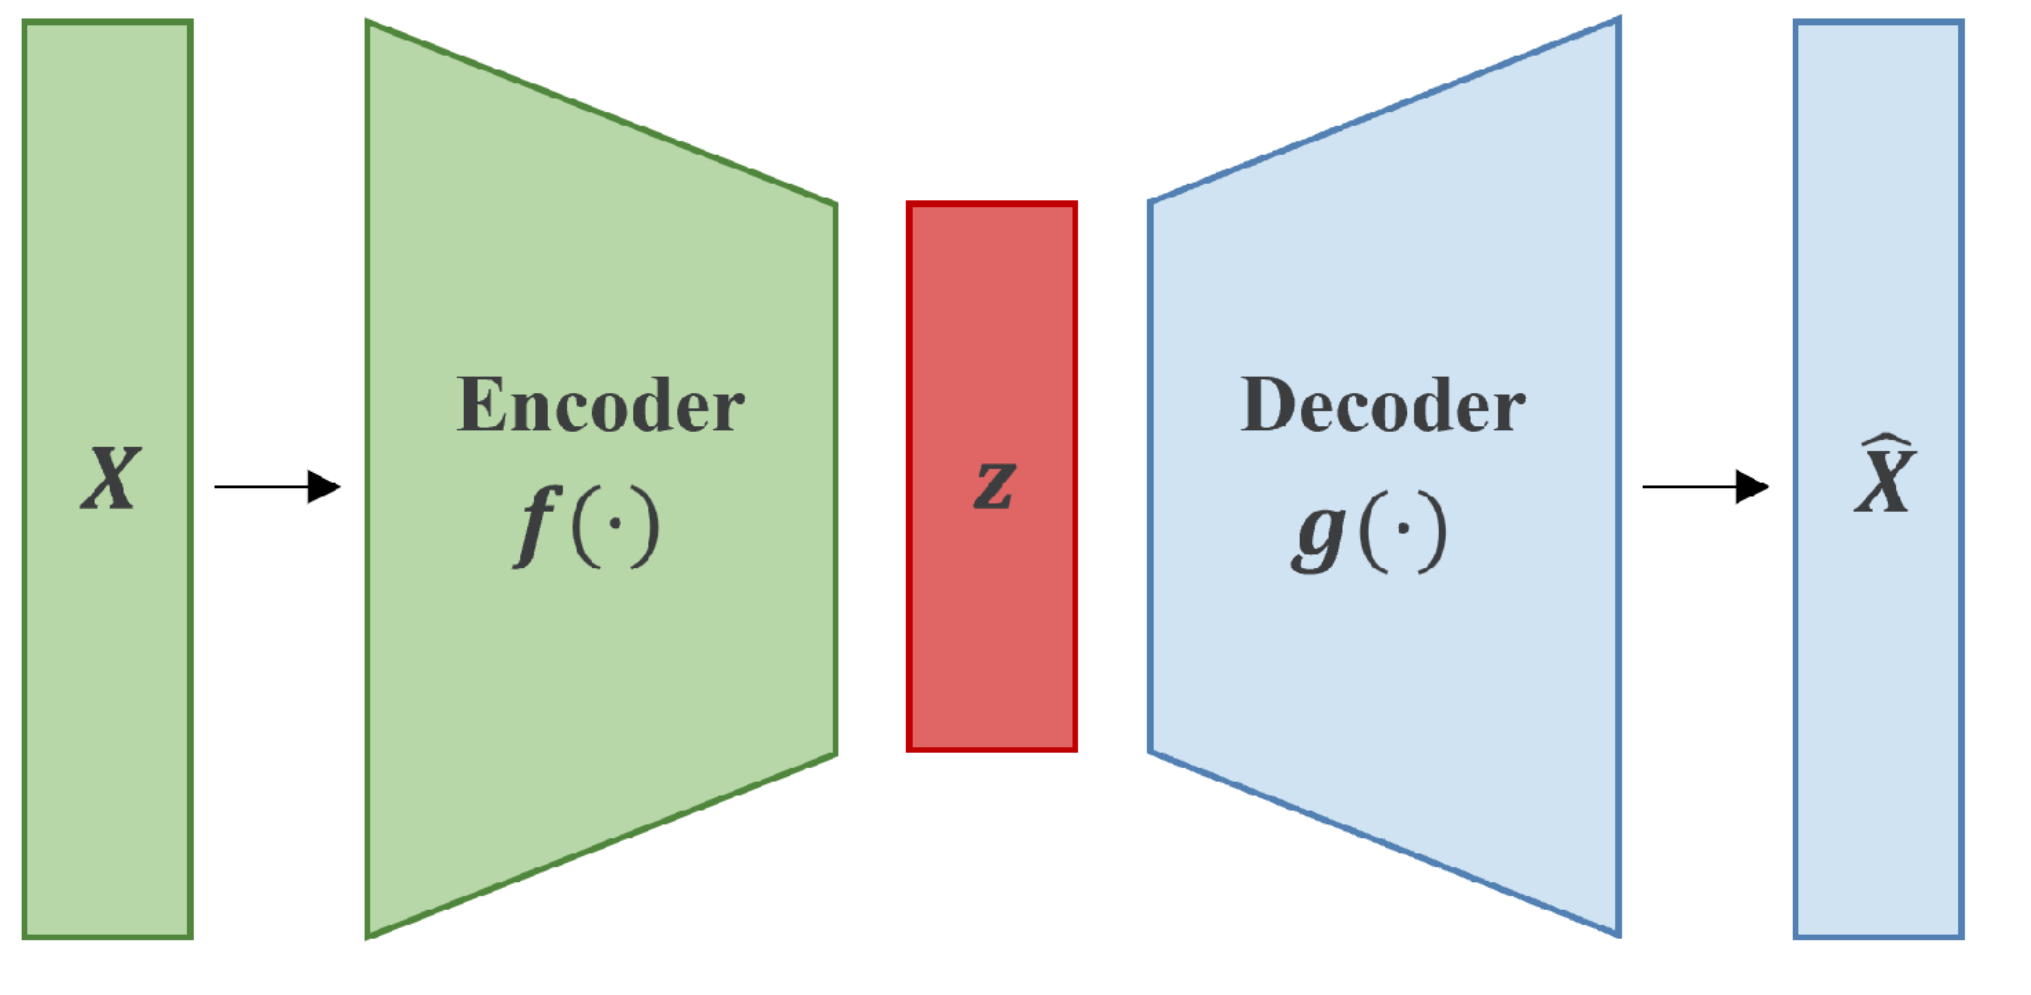
\includegraphics[width=0.6\textwidth]{ae-class.png}
    \caption{Autoencoder(VAE) class}
    \label{fig:ae-class}
\end{figure}

The AE class is a fundamental deep learning model that learns a compressed representation of the input data. The AE consists of an encoder and a decoder, which are trained to minimize the reconstruction error between the input and output.  First a dual branch is used to map $S_t$ and $S_f$ to a latent dimension $E$. Then these latent representations are concatenated and have a dimension of $2E$. An MLP layer is then applied to map the fused vector into dimension $E$, which is the shared bottleneck of both time and frequency domain data's latent space. Finally, two domain specific decoders are used to reconstruct the time and frequency domain signals. In the case of linear autoencoder where we also drop the non-linear operations, the autoencoder would achieve the same latent representation as Principal Component Analysis (PCA). The architecture is shown in \autoref{fig:ae-class}.

\begin{figure}[htbp]
    \centering
    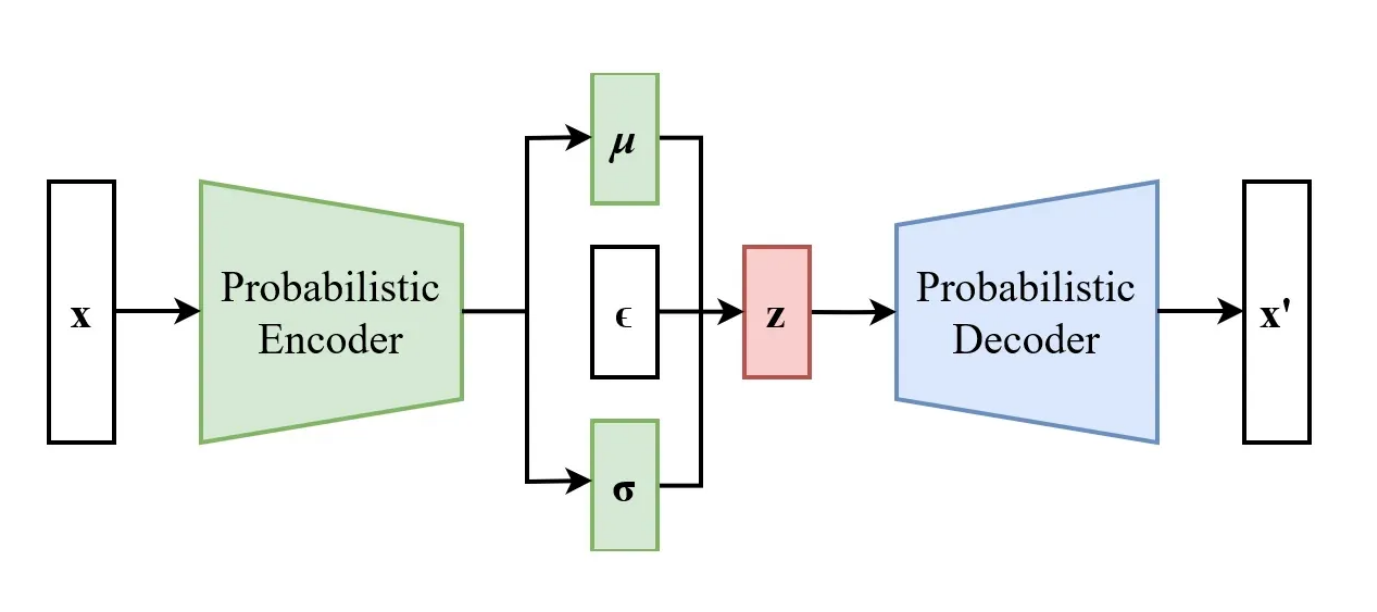
\includegraphics[width=0.5\textwidth]{vae-class.png}
    \caption{Variational Autoencoder(VAE) class}
    \label{fig:vae-class}
\end{figure}


To model the reconstruction error, we use the mean squared error (MSE) loss function:
$$
    L_{\text{AE}} = \frac{1}{N} \sum_{i=1}^{N} \left( \left\| S_{t}^{(i)} - \hat{S}_{t}^{(i)} \right\|_{2}^{2} + \left\| S_{f}^{(i)} - \hat{S}_{f}^{(i)} \right\|_{2}^{2} \right)
$$


The Variational Autoencoder (VAE) extends traditional autoencoders by introducing a probabilistic framework to model the latent space. Unlike deterministic autoencoders, VAEs learn a generative model of the data by approximating the true posterior distribution of latent variables $z$ given the input $x$. This is achieved via an encoder-decoder architecture governed by parameters $\phi$(encoder) and $\theta$ (decoder), as shown in \autoref{fig:vae-class}.

The objective is to maximize the evidence lower bound :
$$
    \text{ELBO}(\theta,\phi;x) = \mathbb{E}_{q_{\phi}(z|x)} \left[ \log p_{\theta}(x|z) \right] -  D_{\text{KL}} \left( q_{\phi}(z|x) || p(z) \right)
$$

Our VAE implementation extends this framework to fuse time-domain $S_t  $ and frequency domain $S_f$ signals. Two domain specific encoders process $S_t$ and $S_f$, produce $h_t$ and $h_f$. Features are concatenated and mapped to latent parameters:
$$
    \mu = f_{\mu}(h_t , h_f) \quad \sigma = f_{\sigma}(h_t , h_f)
$$

The latent vector $z$ is sampled as $z = \mu + \sigma \cdot \epsilon$, where $\epsilon \sim \mathcal{N}(0, I)$ to enable backpropagation. The decoder then reconstructs the input signals from the latent representation. The loss combines reconstruction loss and KL divergence :

$$
    L_{\text{VAE}} = \text{MSE}(S_t, \hat{S_t})+ \text{MSE}(S_f, \hat{S_f}) - \beta \cdot \frac{1}{2} \sum_{i=1}^{d }(1 + \log \sigma_{i}^{2} - \mu_i^{2} - \sigma_i^{2})
$$

The hyperparameter $\beta$ inspired by \todo{Inspired by what } encourages disentangled representations by amplifying the KL term’s regularization effect.

\section{Experiment Results}

\subsection{Data Preprocessing \& Dataset Configuration}

Our experiments leverage the satellite interference dataset from Saif Al-Dawla et al. \cite{saifaldawlaNGSOToGSOSatelliteInterference2023}, comprising 17,281 time-domain magnitude sequences captured from Geostationary (GSO) and Low-Earth Orbit (LEO) satellite links. Table 1 details the dataset splits adhering to the original paper's rigorous simulation setup:

\begin{table}[htbp]
\centering
\caption{Dataset Composition and Splits \cite{saifaldawlaNGSOToGSOSatelliteInterference2023}}
\label{tab:dataset}
\begin{tabular}{lcccc}
\toprule
\textbf{Split} & \textbf{Total Samples} & \textbf{Clean (Class 0)} & \textbf{Interference (Class 1)} & \textbf{SNR Range (dB)} \\
\midrule
Train          & 11,509                 & 11,509                   & 0                                & 6.4--15.4               \\
Validation     & 1,302                  & 1,302                    & 0                                & 6.4--15.4               \\
Test           & 4,470                  & 2,235                    & 2,235                            & 4.5--32.5               \\
\bottomrule
\end{tabular}
\end{table}

Each sample consists of an 800-dimensional time-series magnitude vector derived from DVB-S2X standard transmissions at 100 MHz sampling rate. We preprocess the data as follows:

Normalization: To mitigate amplitude variations from satellite link adaptation, we apply instance-wise standardization:

\begin{align*}
\hat{x}i = \frac{x_i - \mu}{\sigma} \\
\mu = \frac{1}{800}\sum{k=1}^{800} x_k \\
\sigma = \sqrt{\frac{1}{800}\sum_{k=1}^{800} (x_k - \mu)^2}
\end{align*}

\subsection{Models evaluation results}

The proposed framework is rigorously evaluated against a conventional Energy Detection (ED) baseline, which computes the energy threshold $\beta_E$ by optimizing the AUC score on the test dataset. For a received signal $\mathbf{y}_n$, the energy $E_n = \sum_{i=1}^N |y_n[i]|^2$ is compared to $\beta_E$ to detect interference. The ED method achieves 71.67\% accuracy and 0.7167 AUC, with perfect precision (100.0\%) but critically low recall (43.35\%), reflecting its propensity for false negatives under non-Gaussian noise conditions.

Our proposed models—LinearAE, CNNAE, TransformerAE, LinearVAE, CNNVAE, and TransformerVAE—leverage fused time-frequency domain inputs to address these limitations. Architectural variants span linear, convolutional, and transformer-based feature extractors, enabling a systematic exploration of anomaly detection robustness.

As shown in \autoref{tab:model_performance}, CNNAE achieves the highest AUC (0.9175) among all models, surpassing the ED baseline by 20.08\% and demonstrating the efficacy of convolutional architectures in capturing localized interference signatures. The deterministic autoencoder (AE) class consistently outperforms variational autoencoders (VAE), with CNNAE exceeding CNNVAE by 3.51\% in AUC, suggesting that probabilistic latent spaces may introduce unnecessary complexity for this task.

The LinearAE model, despite its simplicity (4.20M parameters), delivers competitive performance (AUC: 0.9176), highlighting the sufficiency of linear projections for interference detection in fused representations. However, its marginally lower recall (81.81\% vs. CNNAE: 81.68\%) underscores the value of hierarchical feature learning in mission-critical scenarios.

In the context of architectural efficiency, LinearAE (4.20M parameters) and LinearVAE(2.4M parameters) achieve near-instant inference (0.0216–0.0253 thresholds), ideal for edge devices with stringent latency constraints.  CNNAE (2.47M parameters) and CNNVAE (2.50M) balance performance and efficiency, requiring 60\% fewer parameters than transformer variants while delivering superior AUC.

As for training dynamics: Transformer architectures exhibit pronounced instability:  TransformerAE collapses entirely (AUC: 0.6690), with training loss oscillations indicating poor convergence.  TransformerVAE struggles to optimize its 27.50M parameters, achieving subpar recall (78.64\%) despite extensive training.

% The AE class outperforms VAE class, suggests that deterministic models are more suitable than probabilistic models. CNNAE achieves the highest AUC score of 91.75\%, outperforming the ED baseline by 20.08\%. LinearAE has the fastest training speed due to its simplicity, but its performance is slightly lower than CNNAE. TransformerAE is particularly hard to converge, with  its training loss oscillating. This shows anomaly detection on interference should not be viewed as a time series modeling problem.

Transformer-based models, despite their theoretical allure, fall short in this context. The TransformerVAE, with its hefty 27M parameters, only manages an 87.3\% AUC, highlighting a clear mismatch between its complexity and the task’s requirements. Even more concerning is the TransformerAE’s convergence issue, which drags its AUC down to a mere 66.9\%. These results suggest that the lack of a strong inductive bias for sequential data makes transformers less suited for interference detection in this setting, where localized features play a dominant role.


\begin{table}[htbp]
    \centering
    \caption{Classification Performance of AE and VAE Models}
    \vspace{5pt}
    \label{tab:model_performance}
    \begin{adjustbox}{width=\textwidth}
        \begin{tabular}{lccccccc}
            \toprule
            \textbf{Model} & \textbf{Threshold} & \textbf{Precision} & \textbf{Recall} & \textbf{F1-Score} & \textbf{Accuracy} & \textbf{AUC} & \textbf{Params(M)} \\
            \midrule

            \multicolumn{8}{l}{\textbf{Autoencoders (AE)}}                                                                                                         \\
            \midrule
            LinearAE       & 0.0216             & 0.8182             & 0.8181          & 0.8181            & 0.8181            & 0.9176       & 4.20               \\
            CNNAE          & 0.0208             & 0.8168             & 0.8168          & 0.8168            & 0.8168            & 0.9175       & 2.47               \\
            TransformerAE  & 0.0013             & 0.5278             & 0.5277          & 0.5277            & 0.5277            & 0.6690       & 10.96              \\

            \midrule
            \multicolumn{8}{l}{\textbf{Variational Autoencoders (VAE)}}                                                                                            \\
            \midrule
            LinearVAE      & 0.0253             & 0.7895             & 0.7895          & 0.7895            & 0.7895            & 0.8860       & 2.40               \\
            CNNVAE         & 0.0255             & 0.7891             & 0.7890          & 0.7890            & 0.7890            & 0.8864       & 2.50               \\
            TransformerVAE & 0.0325             & 0.7864             & 0.7864          & 0.7864            & 0.7864            & 0.8733       & 27.50              \\

            \bottomrule
        \end{tabular}
    \end{adjustbox}

\end{table}

\begin{figure}
    \centering
    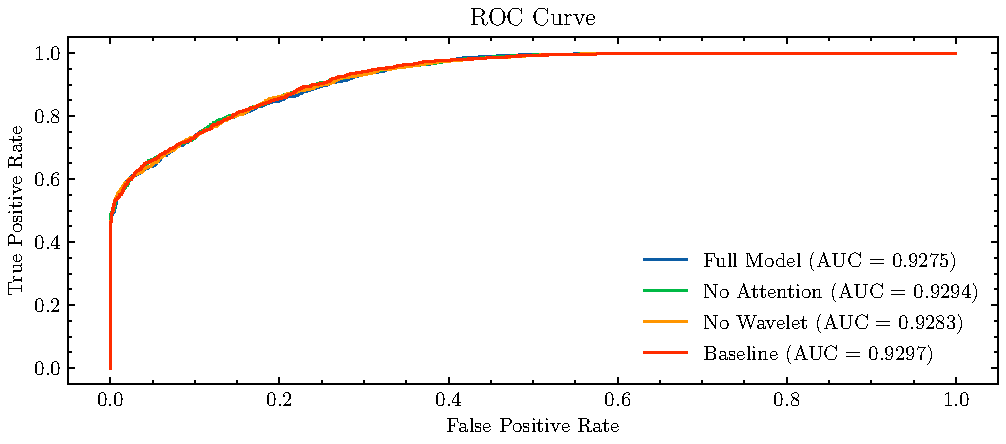
\includegraphics[width=0.8\textwidth]{roc.pdf}
    \caption{Receiver Operating Characteristic (ROC) curves for AE and VAE models}
    \label{fig:roc}
\end{figure}


\begin{figure}[htbp]
    \centering
    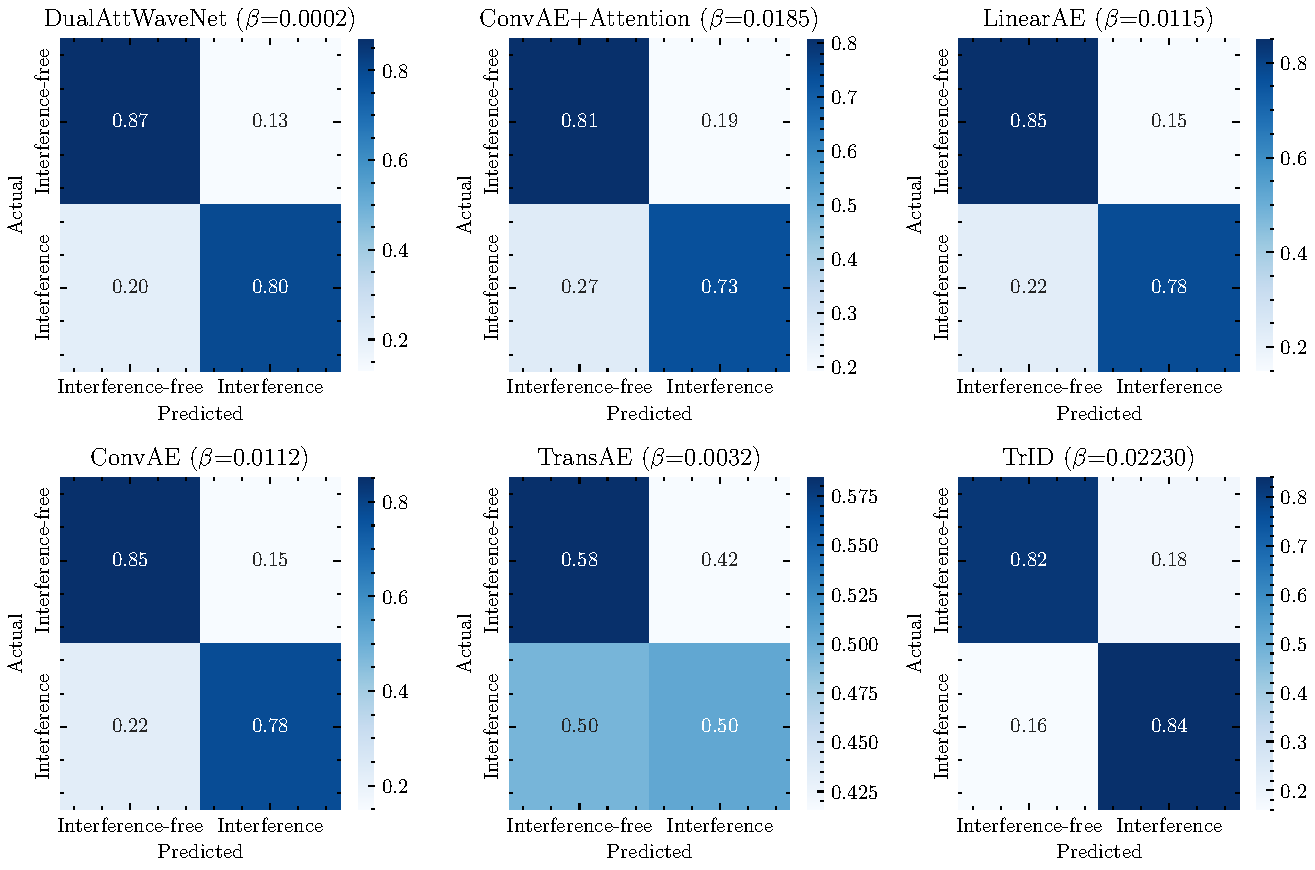
\includegraphics[width=0.8\textwidth]{confusion.pdf}
    \caption{Confusion matrix for AE and VAE models}
    \label{fig:prc}
    
\end{figure}

\medskip

\printbibliography

\end{document}